%!TEX root = main.tex
\section{Experiments}\label{sec:experiments}
\begin{table}[b!]
	\resizebox{1\columnwidth}{!}{%
		\centering\begin{tabular}{clcclllc}\toprule
			&        &                         &                         & Qualification   & Protected & Protected \\
			& Dataset & \multicolumn{1}{c}{$n$} & \multicolumn{1}{c}{$k$} & criterion & groups     & \% \\
			\midrule
			D1 & COMPAS \cite{angwin_2016_machine}& 6173 & 1500 & ad-hoc score & people of color (PoC) & 65.9\% \\
			\midrule
			D2 & COMPAS \cite{angwin_2016_machine}& 6173 & 500 & ad-hoc score & 25yr. < x < 45yr. & 57.2\% \\
			& & & & & < 25yr. & 21.8\% \\
			\midrule
			D3 & COMPAS \cite{angwin_2016_machine}& 6173 & 300 & ad-hoc score & PoC female, < 25yr. & 2.8\%\\
			& & & & & white female, < 25yr. & 1.2\% \\
			& & & & & PoC male, < 25yr. & 13.4\% \\
			\midrule
			D4 & German credit \cite{lichman_2013_uci} & 1000 & 50 & credit rating & female, non-prot. age & 21.7\% \\
			& & & & & male, oldest 10\% & 6.3\% \\
			& & & & & male, youngest 10\% & 4.4\%  \\
			& & & & & female, oldest 10\% & 3.2\% \\
			& & & & & female, youngest 10\% & 6.1\% \\
			\midrule
			D5 & LSAT \cite{wightman1998lsac}  & 21K & 300  & LSAT score  & White, female & 35.3\%  \\
			& & & & & PoC, female & 8.4\% \\
			& & & & & PoC, male & 7.6\% \\
			\bottomrule
		\end{tabular}
	}
	\caption{Datasets and experimental settings. The ad-hoc score for COMPAS was calculated by a weighted summation of recidivism risk, number of prior arrests and violent recidivism risk.	\label{tbl:datasets}}
	\vspace{-3mm}
\end{table}
%
In this section, we evaluate the multinomial \algoFAIR algorithm.
%
We present the datasets we used in \S\ref{sec:experiments-datasets}, metrics and comparison with baselines in \S\ref{sec:experiments-baselines}, and results in \S\ref{sec:experiments-results}.

\begin{figure}[t]
	\vspace{-8mm}
	\centering
	\subfloat%
	[Score distribution of male and female candidates in the COMPAS dataset.
	\label{fig:dataset:compas:sex}]
	{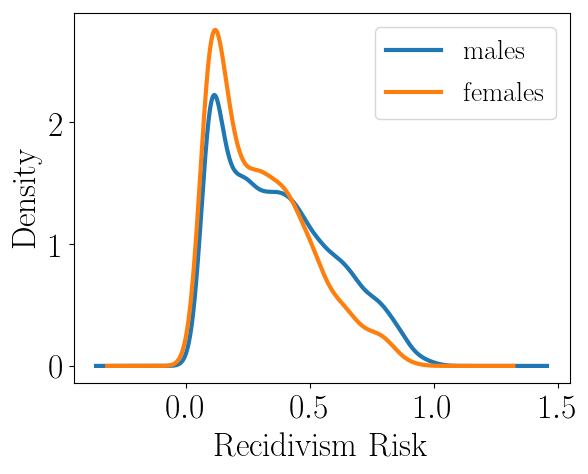
\includegraphics[width=.48\textwidth]{pics/compas_sex_kde.png}}\hfill
	\subfloat
	[Score distribution of white candidates and people of color (PoC) in the COMPAS dataset. Experiment D1.
	\label{fig:dataset:compas:race}]
	{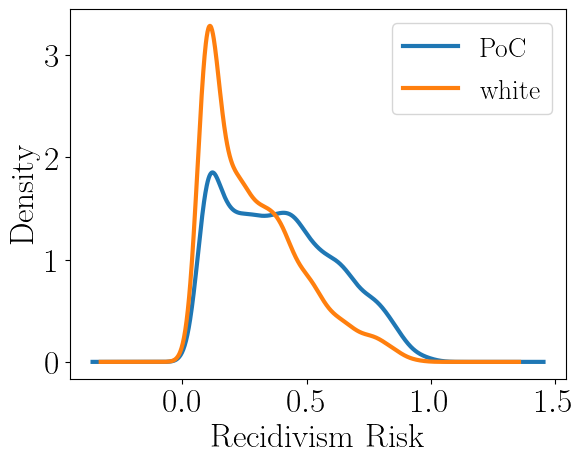
\includegraphics[width=.48\textwidth]{pics/compas_race_kde.png}}\hfill
	\subfloat
	[Score distribution by age in the COMPAS dataset. We see that age is a strong predictor of recidivism risk which suggests that the COMPAS questionnaire injects a bias against younger people into the data. Experiment D2.
	\label{fig:dataset:compas:age}]
	{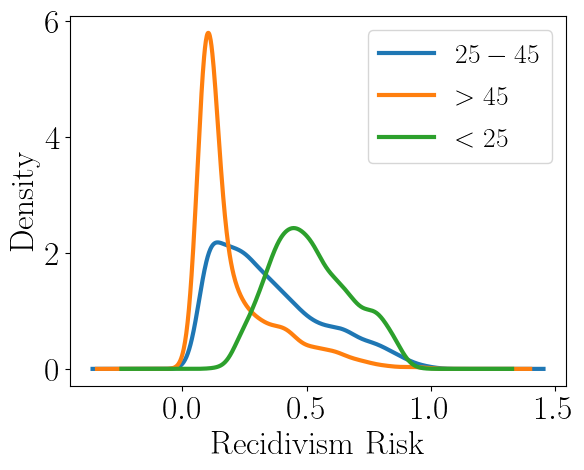
\includegraphics[width=.48\textwidth]{pics/compas_age_kde.png}}\hfill
	\subfloat
	[Score distribution protected and non-protected candidates in the COMPAS dataset. Protected groups are young male PoC, young female PoC and young white females, which are the three groups with lowest average exposure in the colorblind ranking. Experiment D3.
	\label{fig:dataset:compas:worstThree}]
	{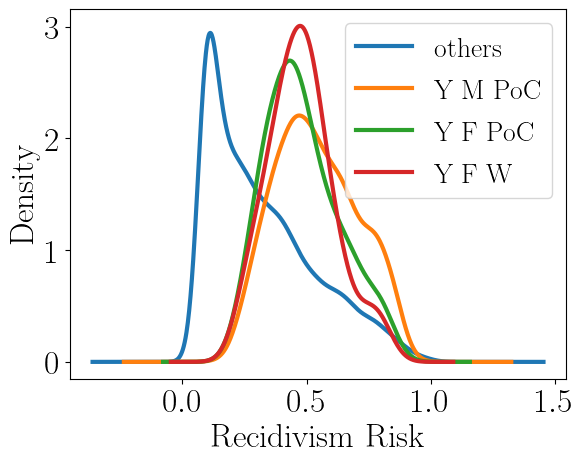
\includegraphics[width=.48\textwidth]{pics/compas_worstThreeGroups_kde.png}}\hfill
	\vspace{-3mm}
	\caption{Distribution of COMPAS scores in different experimental settings. The first three figures show distributions separately by each of the three protected categories. The fourth figure shows the distribution for dataset D3}
	\label{fig:dataset:compas}
\end{figure}

\subsection{Datasets}\label{sec:experiments-datasets}

We used multiple datasets in our experiments, each dataset represents a set of people with certain demographic attributes, and includes a ``score'' attribute.
%
Table~\ref{tbl:datasets} presents some general characteristics of each dataset.
%
Dataset D1 corresponds to the same experimental setup as in our previous work~\cite{zehlike2017fair}, but instead of using the original algorithm \algoFAIR, we run the binomial experiment with the multinomial extension proposed in Section~\ref{sec:problem}.
%
We perform tests with various values of $k<n$ in each dataset.
%
Additionally, we tested different definitions of what would constitute a protected group within each dataset, for experimental purposes.
%
However, we must note that in a real application there is usually a protected group that is clearly defined by voluntary agreements or by law, and that group historically and currently experiences a disadvantage.
%
Similarly, the minimum proportion can always be provided by regulation or voluntary commitments; in the absence of this minimum proportion one can use the fraction of people who are members of that group within the entire population.
%
An experiment consists of generating a ranking from the set of candidates using multinomial \algoFAIR and then comparing it with baseline rankings according to the metrics introduced in the next section.
%
We use the three publicly-available datasets: COMPAS~\cite{angwin_2016_machine}, German Credit~\cite{lichman_2013_uci} and LSAC~\cite{wightman1998lsac}.

\spara{COMPAS} is a criminal recidivism risk assessment instrument that predicts the probability of a convict to recidivate within the two years after the sentence. It is based on a set of over a hundred items or questions, and currently it is used by several jurisdictions in the US.
%
COMPAS has been accused of racial discrimination by having a larger false positive rate for African Americans~\cite{angwin_2016_machine}.
%
In our experiment, we test a scenario in which we want to create a fair ranking of the top-$k$ people who are least likely to recidivate, who could be, for instance, considered for an alternative program to prison.
%
We calculated a candidate's overall score as a weighted summation of the columns ``recidivism, violent recidivism'' and ``prior arrests'' from the original dataset.
%
To break ties, we added normally distributed random noise with $\mu=0, \sigma=0.00001$ to the score of each candidate.
%
Our protected groups are formed by different combination of the attributes ``race, age'' and ``sex'', where race is either ``white'' or ``person of color'' (PoC), age is either ``younger than 25'', ``between 25 and 45'' or ``older than 45'', and sex is either ``male'' or ``female''.
%
We observe in Figure~\ref{fig:dataset:compas} that PoC (\ref{fig:dataset:compas:race}), as well as males (\ref{fig:dataset:compas:sex}) are given a larger recidivism score than other groups.
%
However we see in Figure~\ref{fig:dataset:compas:age} that the protected attribute ``age'' has the strongest impact on recidivism risk.
%
Apparently COMPAS tends to give larger risk scores to younger people.
%
We therefore consider white, female and older than 45 as the \emph{non-protected} categories for our experiments.


In dataset D1 we consider people of color as the protected group and conduct experiments with two different minimum proportion vectors.
%
The first one sets the $p$-values to match the protected group proportion in the dataset $p_{\text{stat}}=[0.66]$ which relates to group fairness as statistical parity; the second one sets all minimum proportions to the same value $p_{\text{eq}}=[0.5]$.


In dataset D2 we consider people aged 25--45 and younger than 25 as protected and the vectors $p_G$ are $p_{\text{stat}}=[0.573,0.218]$ and $p_{\text{eq}}=[0.333, 0.333]$.


In dataset D3 we divided the candidates into 12 different groups that we constructed from the Cartesian product of all three protected categories ``age,'' ``race,'' and ``sex''.
%
Then we calculated the average group exposure for each group and considered as protected the three groups that were placed lowest in the colorblind ranking.
%
These are young female persons of color, young white females and young male PoC.
%
Interestingly, despite the fact that females have higher scores on average, two of the three groups with lowest exposure values are female (Figure~\ref{fig:dataset:compas:worstThree}).
%
We set the vectors $p_G$ to $p_{\text{stat}}=[0.028,0.012,0.134]$ and $p_{\text{eq}}=[0.25,0.25,0.25]$.


\spara{German Credit} is a dataset based on ratings generated by the German agency \emph{Schufa,} and is also known as the Statlog German Credit Dataset.
%
The score given by \emph{Schufa} is based on age, gender, marital status, and other features of each applicant, and is widely used in Germany as a credit rating score for operations such as renting an apartment or applying for a loan.
%
The dataset provides a credit-worthiness score that we use as ``qualification,'' and corresponds to a weighted sum of credit duration, credit amount, and employment length.
%
As protected attributes we use the sex and age of a candidate: females and whether or not they belong to the group of the 100 youngest or oldest persons respectively form the protected groups, because these tend to be given lower scores.
%
We set the vectors $p_G$ to $p_{\text{stat}}=[0.217,0.063,0.044,0.032,0.061]$ and $p_{\text{eq}}=[0.166,0.166,0.166,0.166,0.166]$.


\spara{LSAT} is a dataset collected by~\citet{wightman1998lsac} to study whether the admission metrics to law schools in the US have a disparate impact on students of color.
%
The qualification attribute consists of scores in the US Law School Admission Test (LSAT).
%
The protected features are a person's sex and whether or not they belong to the group of people of color (PoC).
%
Women and PoC score on average lower than men and Whites in this test, which is why we regard white men as non-protected and the other groups as protected.
%
We set the vectors $p_G$ to $p_{\text{stat}}=[0.353,0.084,0.076]$ and $p_{\text{eq}}=[0.25,0.25,0.25]$.


\subsection{Baseline Methods and Metrics}\label{sec:experiments-baselines}

The baseline methods for comparison that we use are the following:

\spara{Baseline 1: Group-unaware or ``color-blind'' ranking.} This method merely order the candidates by decreasing scores/qualifications (see Section~\ref{concept:color-blind-ranking}) \changed{and therefore maximizes selection and ordering utility.
	%
We evaluate all methods relative to the metrics achieved by the colorblind ranking, {\it i.e.}, we report utility loss and fairness gain of the methods w.r.t. the colorblind ranking.}

\spara{Baseline 2: Continuous Fairness Algorithm (CFA$\theta$).} This is a post-processing method introduced by \citet{zehlike2020matching}\changed{, and as explained in Section~\ref{subsec:fair-ranking}, to the best of our knowledge this is the only utility-based method in the literature that does not assume that utilities can be compared across groups}.
%
It aligns the score distributions of the protected candidates with the Wasserstein-barycenter of all group distributions.
%
To achieve this the algorithm finds a new distribution of scores for each group, the "fair representation", by interpolating between the barycenter and the group distribution, subject to a given fairness parameter $\theta$.
%
This fair representation corresponds to the idea to rank groups separately and then subsequently pick the best candidates from each group to create the result ranking.
%
Note that setting $\theta=1$ to its maximum corresponds to setting the minimum proportions in $p_G$ to the dataset proportions of each group.
%
This means that with CFA$\theta$ we cannot achieve an exposure gain that would require minimum proportions beyond statistical parity.
%
Hence this method is comparable to our method only if all values in $p_G$ are less or equal to statistical parity.
%
In our experiments we therefore only compare \algoFAIR with $p_{\text{stat}}$ to CFA$\theta$ with $\theta=1$, as higher $p$-values are not comparable.

\noindent\changed{\spara{Baseline 3: Categorical sampling or ``dice roll''.} We adapt the Bernoulli process of~\citet{yang2016measuring} to a multinomial setting, in which more than one protected group is present.
%
This corresponds to sequentially rolling a $|G|$-sided dice for each of the ranking positions $i=1, 2, \dots, k$, placing at ranking position $i$ the best available candidate from the group whose side is showing (with each candidate appearing at most once in the ranking).
%
Each side of the dice represents one group $g \in G$ and shows with probability $p_g$.
	%
	We note that this procedure, if repeated many times, will approximate the results of \algoFAIR.
	%
	The difference is that our method is deterministic and therefore guarantees a certain share of visibility for each group.
%
We further not that the results we report are only taken w.r.t. one dice rolling experiment, hence another instance may show different utility losses and fairness gains.
}

\spara{Utility (Performance Measure). } We report the loss in ranked utility after score normalization, in which all $q_i$ are normalized to be within $[0, 1]$.
%
We also report the maximum rank drop, {\em i.e.}, the number of positions lost by the candidate that realizes the maximum ordering utility loss.


\spara{NDCG (Performance Measure). }
%
We report a normalized weighted summation (Normalized Discounted Cumulative Gain - NDCG) of the scores of the elements in the ranking, $\sum_{i=1}^{k} w_i q_{(\tau_i)}$, in which the weights are chosen to have a logarithmic discount in the position:  $w_i = \frac{1}{\log_2 (i+1)}$. This is a standard measure to evaluate search rankings~\cite{jarvelin2002cumulated}.
%%
This is normalized so that the maximum value is $1.0$.

\noindent\changed{\spara{Kendall's Tau (Performance Measure). } We report the similarity of the fair candidate orderings w.r.t. the colorblind ranking in terms of Kendall's $\tau$ correlation coefficient.
%
A value close to 1 indicates strong similarity between the two rankings (with 1 meaning perfect agreement), a value close to -1 indicates strong dissimilarity (with -1 meaning perfectly reversed ordering), and a value of 0 indicates there is no correlation between the two rankings.}

\spara{Exposure (Fairness Measure). } We use a measure of average group exposure, which we define as the average position bias that a group is exposed to.
%
In rankings, their exposure to the user is critical for ranked candidates to benefit from the system and if a group of candidates is systematically ranked low, it can be considered as biased~\cite{friedman1996bias}.
%
We model position bias $v$ by means of a logarithmic progression of the form $v(k) = \frac{1}{\log_2(i+1)}$.
%
Thus the first position has a bias $v(1)=1$, which then decreases logarithmically.
%
Higher position bias translates into more exposure and hence more visibility.
%
We show that large increases in average group exposure can be achieved with relatively small losses in ordering utility and NDCG.


\subsection{Results}\label{sec:experiments-results}
%
\begin{table}[t!]
	\caption{Experimental results, showing changes in the average group exposure and ranking utility in terms of NDCG.
		%
		%Colorblind results are not shown because they are always zero.
		%
		Exposure is presented per group while the loss of NDCG is calculated for the entire ranking.
		%
		The protected groups are in the same order as in Table~\ref{tbl:datasets}.
		%
		%With $p_{\text{stat}}$ we denote a vector $p_G$ that contains the share of a group as its $p$-value, hence the produced ranking should obtain statistical parity.
		%
		%With $p_{\text{equal}}$ we denote a vector $p_G$ that contains the same value for all $p$.
		%
		For exposure gain we report numbers with an asterisk, if a group was not among the top-$k$ in the colorblind ranking, but is now.
		%
		These numbers constitute the \emph{absolute} exposure value a group receives after re-ranking.
		%
		Comparable results are grouped together.
		\label{tbl:results-part-one}
	}
	\vspace{-4mm}
	\resizebox{1.02\columnwidth}{!}{%
	\centering\begin{tabular}{llcccc}\toprule
   					&			& Exposure gain 	& Exposure gain		&   total   	& \changed{Kendall's}\\
		Experiment	& Method 	& per prot. group 	& non-prot. group 	& NDCG loss  	& \changed{Tau}\\

		\midrule
		\midrule
		D1 -- COMPAS,	& \algoFAIR $p_{\text{eq}}$ 	& 0.25 	& -0.25 	& 0.0000	& 0.99\\
		k=1500,			& \changed{dice roll} $p_{\text{eq}}$		& -0.45 & 0.45		& 0.0055 	& 0.98\\
						\cline{2-6}
		race (1 prot.)	& \algoFAIR $p_{\text{stat}}$	& 19.77 & -19.77 	& 0.0040 	& 0.82\\
						& \changed{dice roll} $p_{\text{stat}}$	& 28.47 & -28.47	& 0.0070	& 0.77 \\
						& CFA$\theta$ 					& 28.16 & -28.16	& 0.0050	& 0.66\\
		\midrule
		\midrule
		D2 -- COMPAS, 	& \algoFAIR $p_{\text{eq}}$ 	& $[-7.34, 20.87^*]$ 	& -13.53 	& 0.0580 & 0.55 \\
		k=500,			& \changed{dice roll} $p_{\text{eq}}$		& $[-5.07, 21.72^*]$ 	& -16.64	& 0.0585 & 0.51\\
						\cline{2-6}
		age (2 prot.)	& \algoFAIR $p_{\text{stat}}$ 	& $[7.95, 14.11^*]$ 	& -22.06 	& 0.0354 & 0.51 \\
						& CFA$\theta$ 					& $[24.33, 15.91^*]$ 	& -38.48	& 0.0380 & 0.37 \\ %\cline{2-7}
						& \changed{dice roll} $p_{\text{stat}}$	& [8.83, $15.68^*$] 	& -24.52	& 0.0396 & 0.47 \\
		\midrule
		\midrule
		D3 -- COMPAS, 			& \algoFAIR  $p_{\text{eq}}$ 	& $[10.30^*, 10.18^*, 10.25^*]$ & -30.72	& 0.1808 & 0.38 \\
		k=300, 					& \changed{dice roll} $p_{\text{eq}}$		& $[11.60^*, 11.81^*, 11.81^*]$	& -35.21	& 0.2083 & 0.29\\
								\cline{2-6}
		3 worst off (3 prot.)	& \algoFAIR  $p_{\text{stat}}$ 	& $[0.84^*, 0.41^*, 4.08^*]$ 	& -5.33		& 0.0180 & 0.81\\
							 	& CFA$\theta$ 					& $[0.93^*, 0.24^*, 6.74^*]$ 	& -7.92		& 0.0236 & -0.12 \\
								& \changed{dice roll} $p_{\text{stat}}$	& $[2.03^*, 0.59^*, 7.01^*]$	& -9.73		& 0.0353 & 0.69 \\

		\midrule
		\midrule
		D4 -- German credit, 	& \algoFAIR $p_{\text{eq}}$ 	&  $[0.08, 0.50, 1.49, 1.26, 1.12]$ 	& -4.46 &	0.1685	& 0.51 \\
		k=50,					& \changed{dice roll} $p_{\text{eq}}$		& $[-1.09, -0.13, 2.76, 1.28, 1.75]$	& -4.58	& 0.2315 & 0.36\\
								\cline{2-6}
		sex \& age (5 prot.)	& \algoFAIR $p_{\text{stat}}$ 	&  $[0.01, 0.23, 0.38, 0.20, 0.01]$		& -0.83 &	0.0185	& 0.84 \\
								& CFA$\theta$ 					&  $[0.34, -0.93, -0.66, -0.03, 0.28]$ 	& 1.00	& 0.0426	& 0.74 \\
								& \changed{dice roll} $p_{\text{stat}}$	& $[0.89, -1.24, -0.38, -0.33, 0.26]$	& 0.80		& 0.0560 & 0.66 \\

		\midrule
		\midrule
		D5 -- LSAT, 			& \algoFAIR $p_{\text{eq}}$ 	& $[-0.32, 10.71, 10.96]$ 	& -21.35 	& 0.0207 	& 0.08 \\
		k=300, 					& \changed{dice roll} $p_{\text{eq}}$		& $[-6.50, 9.19, 14.69]$	& -17.47	& 0.0263 	& 0.07\\
								\cline{2-6}
		sex \& race (3 prot.)	& \algoFAIR $p_{\text{stat}}$ 	& $[4.00, 4.70, 4.89]$ 		& -13.58 	& 0.0053	& 0.09 \\
							 	& CFA$\theta$ 					& $[-0.74, 1.27, 4.64]$ 	& -5.18		& 0.0009 	& -0.03 \\
								& \changed{dice roll} $p_{\text{stat}}$	& $[-0.16, 3.36, 2.24]$		& -5.44		& 0.0028 	& 0.23 \\

		\bottomrule
	\end{tabular}
	}
\end{table}
%
Table~\ref{tbl:results-part-one} and~\ref{tbl:results-part-two} summarize the results.
%
We report on the result for \algoFAIR using $p_G$ in two different settings, namely as a statistical parity vector i.e. the $p$-values for each group correspond to their respective proportions in the dataset ($p_{\text{stat}}$), and as a vector with all $p$-values being equal ($p_{\text{eq}}$).
%
\changed{We report experimental results for the dice rolling baseline using same probability vectors $p_G$ as for \algoFAIR.}
%
The actual values for $p_G$ are given in the dataset descriptions in Section~\ref{sec:experiments-datasets}.
%
Also remember that results of CFA$\theta$ are only comparable to a \algoFAIR $p_{\text{stat}}$ setting.
%
We therefore group those results together that allow for a meaningful comparison.
%
With the $p_{\text{eq}}$ setting, we illustrate the flexibility of our approach compared to CFA$\theta$, which can achieve statistical parity at maximum.

First, we observe that, for \algoFAIR $p_{\text{stat}}$ and CFA$\theta$, in general changes in NDCG with respect to the color-blind ranking are minor.
%
This can be explained as the utility is dominated by the top positions, which usually do not change dramatically.
%
\changed{However, we see that \algoFAIR outperforms CFA$\theta$ significantly in terms of Kendall's tau, which means that the rankings constructed by CFA$\theta$ have much more ordering inversions w.r.t. the color-blind ranking than those constructed by \algoFAIR. }

Second we see that in experiments D1 and D5 \algoFAIR with $p_{\text{stat}}$ and the baseline CFA$\theta$ seem to perform more or less equally well at first glance.
%
While the former yields better numbers in terms of utility, with the latter the protected groups gain higher exposure.
%
\begin{table}[t!]
	\caption{Experimental results, changes of individual utility loss respect to colorblind results.
		%
		%Colorblind results are not shown because they are always zero.
		%
		All measures are presented per group.
		%
		Groups are in the same order as in Table~\ref{tbl:datasets}, and the first value is always for the non-protected group.
		%
		%With $p_{\text{stat}}$ we denote a vector $p_G$ that contains the share of a group as its $p$-value, hence the produced ranking should obtain statistical parity.
		%
		%With $p_{\text{equal}}$ we denote a vector $p_G$ that contains the same value for all $p$.
		%
		\changed{Experiments that allow for meaningful comparisons are grouped together.}
	}
	\vspace{-4mm}
	\label{tbl:results-part-two}
	\resizebox{1.02\columnwidth}{!}{%
		\centering\begin{tabular}{llccc}\toprule
			& 			& Ordering     & Rank & Selection \\
			Experiment 	& Method 	& utility loss & drop & utility loss \\

			\midrule
			\midrule
			D1 -- COMPAS,	& \algoFAIR $p_{\text{eq}}$ 	& $[0.0066, 0]$ & $[17, 0]$ 	& $[0, 0]$ \\
			k=1500, 		& \changed{dice roll} $p_{\text{eq}}$ 	& $[0.0066, 0.0066]$ & $[60, 30]$ 	& $[0, 0.0066]$ \\
							\cline{2-5}
			race (1 prot.)	& \algoFAIR $p_{\text{stat}}$ 	& $[0.0702, 0]$ & $[387, 0]$ 	& $[0.0621,0]$ \\
							& CFA$\theta$ 					& $[0.0687, 0]$ & $[579, 297]$ 	& $[0.0636, 0]$ \\
							& \changed{dice roll} $p_{\text{stat}}$ 	& $[0.0833, 0]$ & $[524, 0]$ 	& $[0.0833, 0]$ \\

			\midrule
			\midrule
			D2 -- COMPAS, 	& \algoFAIR $p_{\text{eq}}$ 	& $[0.23, 0,23, 0.00]$ & $[182, 116, 0]$ 	& $[0.23, 0.23, 0.00]$ \\
			k=500, 			& \changed{dice roll} $p_{\text{eq}}$ 	& $[0.23, 0.23, 0.00]$ & $[214, 77, 0]$ 	& $[0.23, 0.23, 0.00]$ \\
							\cline{2-5}
			age (2 prot.)	& \algoFAIR $p_{\text{stat}}$ 	& $[0.21, 0.21, 0.00]$ & $[287, 0, 0]$ 		& $[0.21, 0.21, 0.00]$ \\
							& CFA$\theta$ 					& $[0.19, 0.18 ,0.00]$ & $[159, 282, 0]$ 	& $[0.19, 0.17, 0.00]$ \\ %\cline{2-7}
							& \changed{dice roll} $p_{\text{stat}}$ 	& $[0.22, 0.22, 0.00]$ & $[310, 0, 0]$ 		& $[0.22, 0.22, 0.00]$ \\

			\midrule
			\midrule
			D3 -- COMPAS, 			& \algoFAIR  $p_{\text{eq}}$ 	& $[0.60, 0.26, 0.00, 0.37]$ 	& $[206, 0, 0, 0]$ 		& $[0.60, 0.26, 0.00, 0.37]$ \\
			k=300,					& \changed{dice roll} $p_{\text{eq}}$ 	& $[0.63, 0.37, 0.00, 0.49]$ & $[209, 0, 0, 0]$ 	& $[0.71, 0.37, 0.00, 0.49]$ \\
									\cline{2-5}
			3 worst off (3 prot.)	& \algoFAIR  $p_{\text{stat}}$ 	& $[0.17, 0.03, 0.00, 0.02]$ & $[38, 0, 0, 0]$ 				& $[0.17, 0.01,0.01, 0.00] $  \\
								 	& CFA$\theta$ 					& $[0.15, 0.01, 0.00, 0.00] $ & $[268, 0, 0, 0]$ 	& $[0.15, 0.00, 0.00, 0.00]$   \\
									& \changed{dice roll} $p_{\text{stat}}$ 	& $[0.20, 0.001, 0.006, 0.02]$ & $[62, 0, 0, 0]$ 		& $[0.20, 0.01, 0.03, 0.00]$ \\

			\midrule
			\midrule
			D4 -- German credit, 	& \algoFAIR $p_{\text{eq}}$ 	&  $[3.57, 2.70, 3.42, 0.55, 1.23, 1.76]$ 	& $[28, 4, 6, 1, 0, 0]$ 	& $[3.05, 1.82, 1.34, 0.00, 0.18, 0.33]$ \\
			k=50,					& \changed{dice roll} $p_{\text{eq}}$ 	& $[3.65, 5.07, 4.19, 1.05, 1.23, 2.14]$ & $[22, 17, 9, 0, 0, 0]$ 	& $[3.13, 2.27, 1.46, 0.00, 0.25, 0.23]$ \\
									\cline{2-5}
			sex \& age (5 prot.) 	& \algoFAIR $p_{\text{stat}}$ & $[1.84, 1.56, 0.45, 0.00, 0.33, 1.28]$ & $[5, 3, 1, 0, 0, 5]$ & $[1.89, 1.56, 1.23, 0.00, 1.18, 1.54]$  \\
									& CFA$\theta$ &  $[0.50, 0.91, 2.07, 1.46, 0.72, 0.00]$ & $[2, 1, 32, 14, 2, 0]$ & $[0.34, 0.00, 1.93, 2.20, 0.00, 0.00]$ \\
									& \changed{dice roll} $p_{\text{stat}}$ 	& $[0.92, 0.54, 1.76, 2.55, 0.00, 0.29]$ & $[1, 0, 15, 38, 0, 0]$ 		& $[0.96, 0.56, 2.74, 0.00, 2.92, 0.20]$ \\

			\midrule
			\midrule
			D5 -- LSAT, 			& \algoFAIR $p_{\text{eq}}$ 	& $[4, 4, 1, 0]$	& $[220, 10, 0, 0]$ & $[4, 3, 0, 0]$  \\
			k=300, 					& \changed{dice roll} $p_{\text{eq}}$ 	& $[5, 5, 2, 0]$ & $[194, 81, 0, 0]$ 	& $[5, 5, 1, 0]$ \\
									\cline{2-5}
			sex \& race (3 prot.) 	& \algoFAIR $p_{\text{stat}}$ 	& $[2, 2, 1, 0]$ 	& $[136, 13, 0, 0]$ & $[2, 1, 0, 0]$  \\
									& CFA$\theta$ 					& $[1, 1, 1, 0]$ 	& $[122, 26, 0, 0]$ & $[1, 0, 0, 0]$  \\
									& \changed{dice roll} $p_{\text{stat}}$ 	& $[2, 2, 1, 0]$ & $[75, 12, 0, 0]$ 	& $[2, 1, 0, 0]$ \\
			\bottomrule
		\end{tabular}
	}
\end{table}
%
Nonetheless, we found a very important drawback in the results of CFA$\theta$ in experiment D2: \citet{zehlike2020matching} does not guarantee in-group monotonicity, which we observed in our experiments.
%
Consider Table~\ref{tbl:results-part-two} where we observe a maximum rank drop for the non-protected group of 159 for CFA$\theta$, which at first glance is less than \algoFAIR with $p_{\text{stat}}$ (287).
%
However, we found the following problems when closely investigating the result: the candidate that experienced the drop in 159 ranks was the \emph{only non-protected} candidate left in the top-500 after applying CFA$\theta$, and their original ranking position was 341 (now 500).
%
This means that the originally best candidate from the non-protected group (rank 3 in $cb|_k$) was ranked out of the top-500 by CFA$\theta$, hence the in-group ordering is not preserved.
%
We suspect that this is because the method cannot handle ties well.  % RIC: This is not very formal
%
If lots of candidates have very similar original scores, the fair representation scores may have large ties in which candidates are ordered randomly and not w.r.t. their original ordering.
%
In such a setting, \algoFAIR has an important advantage: it guarantees in-group monotonicity, because candidates are separated into group rankings which are sorted by decreasing \emph{original} qualifications.
%
No matter which group has to be picked at the current position, the respective candidate will always be the best available from that group.
%
This means that while very similar scores appear to be problematic for CFA$\theta$, they are the best-scenario for \algoFAIR, because ranked-group fairness can be ensured without losing any relevance at all (NDCG stays unaffected).
%
\changed{This problem also explains the large differences between the methods in terms of Kendall's Tau.}

Third we observe a formerly known weakness of CFA$\theta$ manifesting in experiment D4: it cannot handle data sets with very small groups or groups that show low variance.
%
It increases the exposure of the non-protected group while decreasing it for the oldest males, and youngest males and females.
%
In contrast, \algoFAIR $p_{\text{stat}}$ can handle very small groups, and gives them sufficient exposure that is in line with the minimum proportions $p_G$.
%
For experiment D4 we observe an interesting advantage of \algoFAIR: the youngest and oldest males experience a high rank drop (31 and 22) with CFA$\theta$ compared to \algoFAIR $p_{\text{stat}}$, even though they belong to the protected groups.
%
This is because they receive exposure values higher than average in the $cb|_k$, i.e. these two groups have the best scores.
%
CFA$\theta$ moves \emph{all} score distributions towards the barycenter and thus, removes the advantage that the protected groups have in this data set.
%
\algoFAIR, in contrast, ranks candidates based on their scores, as soon as the ranked group fairness conditions are met for each group.
%
As such, a protected group can only lose exposure for another protected group, but never for the non-protected one.

\changed{When considering the categorical sampling or ``dice rolling'' baseline, we see our expectations of non-consistent behavior confirmed.
	%
	This can be explained by the involved randomness of the dice rolling procedure.
	%
	We observe that in experiments D2 and D3 \algoFAIR $p_\text{eq}$ and \emph{dice roll} $p_\text{eq}$ yield very similar results.
	%
	However in experiments D4 and D5 \algoFAIR $p_\text{stat}$ and \emph{dice roll} $p_\text{stat}$ yield very different results, even though the underlying stochastic process of the two methods is the same.
	%
	In contrast to a dice rolling process, \algoFAIR constructs fair rankings in a deterministic way and therefore always guarantees a minimum representation for each protected group. }

\spara{A wide range of possibilities to set $p_G$.}
%
An important advantage of \algoFAIR is, that it allows to create rankings for user-defined values of $p$ and in particular for values beyond statistical parity, something that cannot be done directly with CFA$\theta$ (\citet{zehlike2020matching} allows at maximum statistical parity in the result ranking when setting $\theta=1$, {\it i.e.}, to the maximum value).

Figure~\ref{fig:results-moving-p} shows results when varying $p_1$ and $p_2$ in data set D2: COMPAS, the protected groups are people of age 25--45 ($p_1$) and people under 25 years ($p_2$).
%
In Fig.~\ref{fig:experiments:compasAge:expGain:groupNP} we see that the non-protected group loses exposure under all settings, as expected.
%
At the same time however NDCG loss is minor and under many settings not increasing beyond a statistical significance level of 0.05\% (Fig.~\ref{fig:experiments:compasAge:ndcgloss}).
%
Comparing Figures~\ref{fig:experiments:compasAge:expGain:group1} and~\ref{fig:experiments:compasAge:expGain:group2} we see that in general, if one protected group scores significantly better in the colorblind ranking (group ``25 -- 45'' in Fig.~\ref{fig:dataset:compas:age}) than another one (group ``younger 25'' in Fig.~\ref{fig:dataset:compas:age}), the first may be ranked down to make room for the second.
%
Figure~\ref{fig:experiments:compasAge:expGain:group1} shows that the middle-aged group in the COMPAS data set loses exposure to the young group unless $p_1$ is set high enough.
%
However even if $p_1$ is set low it still ensures that candidates from the middle-aged group show in the ranking, thus always losing less exposure than the non-protected group (compare Fig.~\ref{fig:experiments:compasAge:expGain:groupNP} and~\ref{fig:experiments:compasAge:expGain:group1}).
%
Note that this experiment is an extreme case, where no candidates from group ``age < 25'' where ranked in the top-200 in $cb|_k$, which explains why this group never loses exposure under any setting for $p_1$ and $p_2$ (see Fig.~\ref{fig:experiments:compasAge:expGain:group2}).

This experiment shows that \algoFAIR allows a wide range of positive actions, for instance, granting reintegration programs to people with promising COMPAS ratings, with a preference towards younger offenders.
%
In this case, the Figure~\ref{fig:experiments:compasAge:ndcgloss} shows that we can double the proportion of young people in the top-$k$ ranking (e.g. from 0\% in the original up to 40\% in the fair ranking) without introducing a large drop for the other protected group loss: in the colorblind ranking they received exposure equivalent to $0.4 > p_1 > 0.5$, so setting $p_1 = p_2 = 0.4$ only causes an exposure drop of 5.8\%.
%
At the same time the NDCG loss is just 5.6\% and never exceeds 15\%, even when favoring young people with $p_2=0.8$.
%
